\section{Why Do We Care About Manifolds? A Concrete Example}
    \label{sec:why_manifolds}

    \subsection{A Real-World Motivation: Temperature on Earth}
    \noindent
    \begin{minipage}[c]{0.62\textwidth}
        Consider our planet modeled as a unit 2-sphere in Euclidean 3-space:
        \begin{equation}
            S^2 = \{ x \in \mathbb{R}^3 \mid \|x\| = 1 \}.
        \end{equation}
        Suppose we measure the surface temperature at every point on Earth.
        This defines a continuous (and physically smooth) scalar function:
        \begin{equation}
            f \colon S^2 \to \mathbb{R}.
        \end{equation}
    \end{minipage}\hfill
    \begin{minipage}[c]{0.35\textwidth}
        \centering
        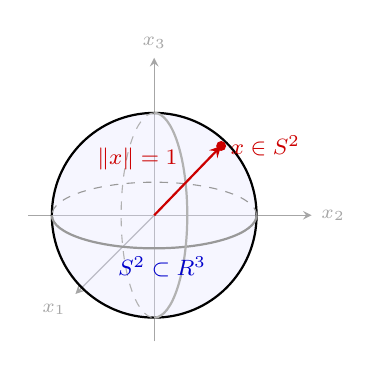
\begin{tikzpicture}[scale=1.0, >=stealth]
  % 3D axes
  \draw[->, gray!70] (-1.6, 0) -- (2.0, 0) node[right, font=\scriptsize] {$x_2$};
  \draw[->, gray!70] (0, -1.6) -- (0, 2.0) node[above, font=\scriptsize] {$x_3$};
  \draw[->, gray!70] (0,0) -- (-1.0, -1.0) node[below left, font=\scriptsize] {$x_1$};
  
  % Sphere
  \draw[thick, fill=blue!10, fill opacity=0.35] (0,0) circle (1.3);
  % Equator
  \draw[dashed, gray!80] (1.3,0) arc (0:180:1.3 and 0.42);
  \draw[thick, gray!80] (-1.3,0) arc (180:360:1.3 and 0.42);
  % Meridian
  \draw[dashed, gray!60] (0,1.3) arc (90:270:0.42 and 1.3);
  \draw[thick, gray!60] (0,1.3) arc (90:-90:0.42 and 1.3);
  
  % Point x on sphere and radius vector
  \draw[->, thick, red!80!black] (0,0) -- (0.85, 0.88) node[midway, above left, font=\footnotesize] {$\|x\|=1$};
  \fill[red!80!black] (0.85, 0.88) circle (1.8pt) node[right, font=\footnotesize] {$x \in S^2$};
  \node[font=\footnotesize, text=blue!80!black] at (0.1, -0.65) {$S^2 \subset \mathbb{R}^3$};
\end{tikzpicture}

    \end{minipage}
    \vspace{0.8em}

    If our goal is purely local, ordinary multivariable calculus from
    Section~\ref{sec:preliminaries} works without issue. However, once we
    study the global behavior of this function across the planet, standard
    calculus in $\mathbb{R}^3$ fails:
    \begin{enumerate}
        \item \textbf{$S^2$ is not an open subset of $\mathbb{R}^3$}:\\
            The standard partial derivative is not defined.
        \item \textbf{Valid directional derivatives must be tangential}:\\
            A legitimate derivative on Earth must measure rates of change
            along directions that are tangent to the surface, rather than
            pointing into the Earth's interior or out into space.
    \end{enumerate}
    That is where manifolds come into place: we need a framework to perform
    calculus directly on curved spaces.

    \subsection{The Intuition: Local Euclidean Approximation}
    The central intuition of a manifold is \textbf{local approximation}. At
    any point $p \in S^2$, a sufficiently small neighborhood $U \subset S^2$
    around $p$ looks like an open region in a flat Euclidean plane
    $\mathbb{R}^2$.

    \begin{figure}[htbp]
        \centering
        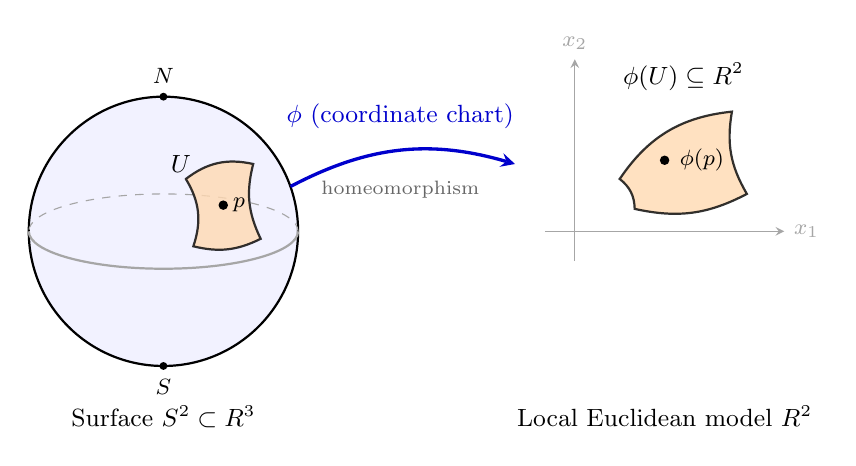
\begin{tikzpicture}[scale=0.95, >=stealth]
  % Left: Sphere S^2
  \begin{scope}[shift={(0,0)}]
    % Sphere outline
    \draw[thick, fill=blue!5] (0,0) circle (1.8);
    % Equator (front solid, back dashed)
    \draw[dashed, gray!70] (1.8,0) arc (0:180:1.8 and 0.5);
    \draw[thick, gray!70] (-1.8,0) arc (180:360:1.8 and 0.5);
    % North and South labels
    \node[above, font=\footnotesize] at (0, 1.85) {$N$};
    \fill (0,1.8) circle (1.5pt);
    \node[below, font=\footnotesize] at (0, -1.85) {$S$};
    \fill (0,-1.8) circle (1.5pt);

    % Local open patch U on sphere
    \draw[thick, fill=orange!30, opacity=0.8] 
      (0.3, 0.7) to[bend left=25] (1.2, 0.9) 
      to[bend right=20] (1.3, -0.1) 
      to[bend left=20] (0.4, -0.2) 
      to[bend right=25] cycle;
    \node[above left, font=\small] at (0.5, 0.65) {$U$};
    \fill (0.8, 0.35) circle (1.8pt) node[right, font=\footnotesize] {$p$};
    \node[below, font=\small] at (0, -2.2) {Surface $S^2 \subset \mathbb{R}^3$};
  \end{scope}

  % Middle: Coordinate chart map phi
  \draw[->, very thick, blue!80!black] (1.7, 0.6) to[bend left=22] 
    node[above=4pt, font=\small] {$\phi$ (coordinate chart)} 
    node[below=7pt, font=\scriptsize, text=gray!80!black] {homeomorphism} (4.7, 0.9);

  % Right: Flat open set in R^2
  \begin{scope}[shift={(5.5,0)}]
    % Axes - crossing at (0,0), clear of the region
    \draw[->, gray!70, thin] (-0.4, 0) -- (2.8, 0) node[right, font=\footnotesize] {$x_1$};
    \draw[->, gray!70, thin] (0, -0.4) -- (0, 2.3) node[above, font=\footnotesize] {$x_2$};
    
    % Flat open region phi(U) placed cleanly in the positive quadrant away from axes
    \draw[thick, fill=orange!30, opacity=0.8] 
      (0.6, 0.7) to[bend left=25] (2.1, 1.6) 
      to[bend right=20] (2.3, 0.5) 
      to[bend left=20] (0.8, 0.3) 
      to[bend right=25] cycle;
      
    % Region label placed comfortably above
    \node[above, font=\small] at (1.45, 1.75) {$\phi(U) \subseteq \mathbb{R}^2$};
    
    % Point phi(p) with label placed centered horizontally inside the orange patch
    \fill (1.2, 0.95) circle (1.8pt) node[right=2pt, font=\footnotesize] {$\phi(p)$};
    
    \node[below, font=\small] at (1.2, -2.2) {Local Euclidean model $\mathbb{R}^2$};
  \end{scope}
\end{tikzpicture}

        \caption{%
            The local coordinate chart: an open neighborhood $U$ on the sphere
            $S^2$ is mapped homeomorphically to an open set $\phi(U) \subseteq
            \mathbb{R}^2$, allowing local calculus on the surface.
        }
        \label{fig:sphere_chart}
    \end{figure}

    \paragraph{Analogy with Algebraic Varieties.}
    An algebraic variety is not globally affine; it is constructed by gluing
    together affine open subsets along regular transition functions.

    \subsection{Constructing \texorpdfstring{$S^2$}{S²} by Gluing Two Disks}
    \label{sec:gluing_s2}

    Here is the picture to keep in mind:
    \begin{enumerate}
        \item Cut one disk from each of two parallel planes.
        \item Bend the disks into two bowls.
        \item Bring the bowls together so they overlap along a narrow strip.
    \end{enumerate}

    \begin{figure}[htbp]
        \centering
        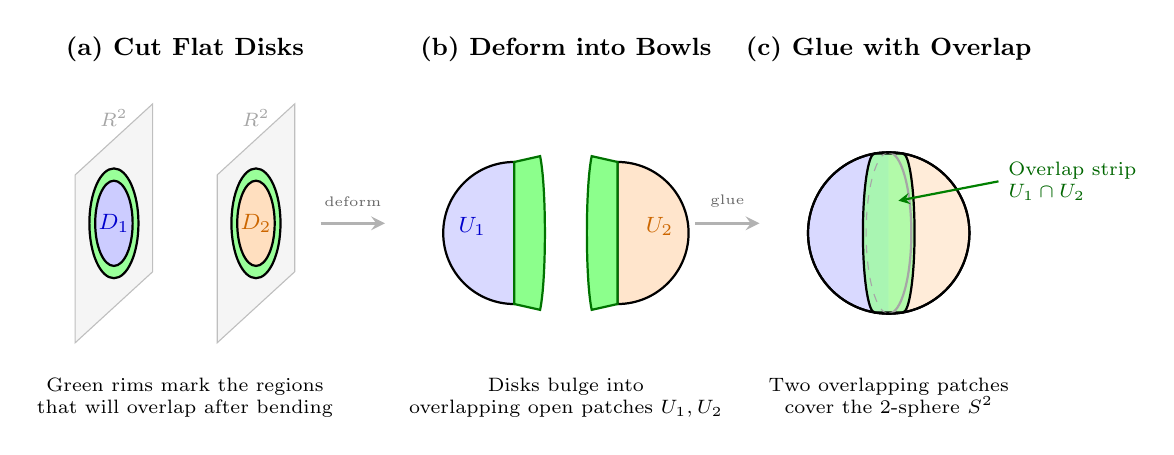
\begin{tikzpicture}[scale=0.82, >=stealth]
  % -------------------------------------------------------------
  % Panel 1: Cut two disks from parallel planes
  % -------------------------------------------------------------
  \begin{scope}[shift={(0,0)}]
    \node[above, font=\bfseries\small] at (1.3, 2.5) {(a) Cut Flat Disks};
    
    % Left plane
    \draw[gray!50, fill=gray!8] (-0.4, -1.7) -- (0.8, -0.6) -- (0.8, 2.0) -- (-0.4, 0.9) -- cycle;
    \node[above, gray!70, font=\scriptsize] at (0.2, 1.5) {$\mathbb{R}^2$};
    % Left disk with a green rim marking the future overlap collar
    \draw[thick, fill=green!40] (0.2, 0.15) ellipse (0.38 and 0.85);
    \draw[thick, fill=blue!20] (0.2, 0.15) ellipse (0.29 and 0.66);
    \node[font=\footnotesize, text=blue!80!black] at (0.2, 0.15) {$D_1$};
    \coordinate (chart-D1) at (0.55,0.15);

    % Right plane
    \draw[gray!50, fill=gray!8] (1.8, -1.7) -- (3.0, -0.6) -- (3.0, 2.0) -- (1.8, 0.9) -- cycle;
    \node[above, gray!70, font=\scriptsize] at (2.4, 1.5) {$\mathbb{R}^2$};
    % Right disk with a matching future overlap collar
    \draw[thick, fill=green!40] (2.4, 0.15) ellipse (0.38 and 0.85);
    \draw[thick, fill=orange!25] (2.4, 0.15) ellipse (0.29 and 0.66);
    \node[font=\footnotesize, text=orange!80!black] at (2.4, 0.15) {$D_2$};
    \coordinate (chart-D2) at (2.75,0.15);

    \node[below, font=\scriptsize, align=center] at (1.3, -2.1) {Green rims mark the regions\\that will overlap after bending};
  \end{scope}

  % Arrow 1 -> 2
  \draw[->, very thick, gray!60] (3.4, 0.15) -- (4.4, 0.15) node[midway, above=2pt, font=\tiny, text=gray!80!black] {deform};

  % -------------------------------------------------------------
  % Panel 2: Deform into overlapping open patches
  % -------------------------------------------------------------
  \begin{scope}[shift={(6.2,0)}]
    \node[above, font=\bfseries\small] at (1.0, 2.5) {(b) Deform into Bowls};

    % Surface strips match the patches in sphere_transition.tex.
    \draw[thick, fill=blue!15]
      (0.2, 1.1) arc (90:270:1.1 and 1.1) -- cycle;
    \path[fill=green!45, draw=green!45!black, thick]
      (0.2,1.1) -- (0.2,-1.1) -- (0.60,-1.19)
      .. controls (0.70,-0.73) and (0.70,0.73) .. (0.60,1.19) -- cycle;
    \node[font=\footnotesize, text=blue!80!black] at (-0.45, 0.1) {$U_1$};
    \coordinate (chart-U1) at (0.0,0.9);
    \coordinate (transition-U1) at (0.5,0.15);

    \draw[thick, fill=orange!20]
      (1.8, 1.1) arc (90:-90:1.1 and 1.1) -- cycle;
    \path[fill=green!45, draw=green!45!black, thick]
      (1.8,1.1) -- (1.8,-1.1) -- (1.40,-1.19)
      .. controls (1.30,-0.73) and (1.30,0.73) .. (1.40,1.19) -- cycle;
    \node[font=\footnotesize, text=orange!80!black] at (2.45, 0.1) {$U_2$};
    \coordinate (chart-U2) at (2.4,0.8);
    \coordinate (transition-U2) at (1.5,0.15);

    \node[below, font=\scriptsize, align=center] at (1.0, -2.1) {Disks bulge into\\overlapping open patches $U_1, U_2$};
  \end{scope}

  % Arrow 2 -> 3
  \draw[->, very thick, gray!60] (9.2, 0.15) -- (10.2, 0.15) node[midway, above=2pt, font=\tiny, text=gray!80!black] {glue};

  % -------------------------------------------------------------
  % Panel 3: Glued together with overlapping strip
  % -------------------------------------------------------------
  \begin{scope}[shift={(12.2,0)}]
    \node[above, font=\bfseries\small] at (0, 2.5) {(c) Glue with Overlap};

    % Left hemisphere (blue)
    \draw[thick, fill=blue!15] (0, 1.25) arc (90:270:1.25);
    
    % Right hemisphere (orange)
    \draw[thick, fill=orange!15] (0, 1.25) arc (90:-90:1.25);

    % Overlapping collar / strip in center (green tint)
    \draw[thick, fill=green!40, fill opacity=0.75] 
      (-0.22, 1.23) arc (90:270:0.18 and 1.23) 
      -- (0.22, -1.23) arc (-90:90:0.18 and 1.23) -- cycle;
      
    % Central boundary curve
    \draw[dashed, gray!70] (0, 1.25) arc (90:270:0.35 and 1.25);
    \draw[thick, gray!70] (0, 1.25) arc (90:-90:0.35 and 1.25);

    % Full sphere circle boundary
    \draw[thick] (0,0) circle (1.25);

    % Callout for overlap placed clearly outside the sphere to the right
    \draw[->, thick, green!50!black] (1.7, 0.8) -- (0.15, 0.5);
    \node[right, font=\scriptsize, align=left, text=green!40!black] at (1.7, 0.8) {Overlap strip\\$U_1 \cap U_2$};

    \node[below, font=\scriptsize, align=center] at (0, -2.1) {Two overlapping patches\\cover the 2-sphere $S^2$};
  \end{scope}

  % The chart-map slide enables these arrows; the original figure omits them.
  \ifdefined\showchartmaps
    \draw[->, very thick, blue!80!black]
      (chart-U1) .. controls +(-0.4,1.8) and +(0.8,2.4) .. (chart-D1)
      node[midway, above=4pt, font=\small] {$\phi_1$};
    \draw[->, very thick, orange!80!black,
        preaction={draw=white,line width=3.5pt}]
      (chart-U2) .. controls +(-1.0,1.9) and +(1.0,2.2) .. (chart-D2)
      node[midway, above=4pt, font=\small] {$\phi_2$};
  \fi

  % A separate variant traces one point through a coordinate transition.
  \ifdefined\showtransitionmaps
    \draw[->, very thick, blue!80!black, shorten <=3pt, shorten >=3pt]
      (chart-D1) .. controls +(0.9,2.2) and +(-0.2,2.2) .. (transition-U1)
      node[midway, above=4pt, font=\small] {$\phi_1^{-1}$};
    \draw[->, very thick, orange!80!black, shorten <=3pt, shorten >=3pt,
        preaction={draw=white,line width=3.5pt}]
      (transition-U2) .. controls +(-0.3,2.0) and +(1.0,2.4) .. (chart-D2)
      node[midway, above=4pt, font=\small] {$\phi_2$};
    \draw[densely dashed, thick, red!80!black, shorten <=4.5pt, shorten >=4.5pt]
      (transition-U1) -- (transition-U2);
    \draw[->, very thick, red!80!black, shorten <=3pt, shorten >=3pt]
      (chart-D1) .. controls +(0.3,-1.65) and +(0.6,-1.65) .. (chart-D2)
      node[midway, below=3pt, font=\small] {$\phi_2\circ\phi_1^{-1}$};
    \foreach \point in {chart-D1,transition-U1,transition-U2,chart-D2}
      \filldraw[fill=red!85!black,draw=white,line width=0.35pt]
        (\point) circle[radius=2.2pt];
    \node[below=10pt,font=\scriptsize,text=red!80!black] at (transition-U1) {$p$};
    \node[below=10pt,font=\scriptsize,text=red!80!black] at (transition-U2) {$p$};
  \fi
\end{tikzpicture}

        \caption{%
            A three-step picture of gluing two disks to form $S^2$. The green
            rims in (a) mark the regions that will overlap after bending.
        }
        \label{fig:sphere_gluing}
    \end{figure}

    \subsection{The Precise Definition of a Smooth Manifold}
    We follow Lee's presentation in Chapter~1, Section ``Smooth Structures,''
    especially pages 11--13 \cite[Chapter~1, ``Smooth Structures,'' pp.~11--
    13]{lee2013smooth}; see also Tu's treatment in Chapter~2
    \cite[Chapter~2]{tu2011introduction}.

    \begin{definition}[Smooth Manifold \cite{lee2013smooth, tu2011introduction}]
        Let $M$ be a Hausdorff, second-countable topological space. These are
        technical assumptions that we will not discuss further; if you are
        unfamiliar with topology, you may think of $M$ as a subspace of some
        $\mathbb{R}^m$.

        A \textbf{coordinate chart} on $M$ is a pair $(U, \phi)$, where $U
        \subseteq M$ is open and $\phi \colon U \to \phi(U) \subseteq
        \mathbb{R}^n$ is a homeomorphism (a continuous bijection with a
        continuous inverse) onto an open subset of $\mathbb{R}^n$.

        Two charts $(U, \phi)$ and $(V, \psi)$ are \textbf{smoothly
        compatible} if either $U \cap V = \emptyset$, or the transition map
        \begin{equation}
            \psi \circ \phi^{-1} \colon \phi(U \cap V) \to \psi(U \cap V)
        \end{equation}
        is a $C^\infty$ diffeomorphism between open subsets of $\mathbb{R}^n$.

        A \textbf{smooth atlas} $\mathcal{A}$ on $M$ is a collection of
        smoothly compatible charts $\{(U_\alpha, \phi_\alpha)\}_{\alpha \in
        I}$ whose domains cover $M$:
        \begin{equation}
            \bigcup_{\alpha \in I} U_\alpha = M.
        \end{equation}
        A \textbf{smooth $n$-manifold} is a Hausdorff, second-countable
        topological space $M$ together with a smooth atlas of dimension $n$.
    \end{definition}

    \subsection{Checking the Gluing Example Against the Definition}

    Return to Figure~\ref{fig:sphere_gluing}. It shows the two bowl-shaped
    patches and the band where they overlap. In
    Figure~\ref{fig:sphere_transition}, the same overlap is drawn on both
    patches: the green strip on the left patch corresponds to the green strip
    on the right. The arrows show points in one strip mapping to corresponding
    points in the other. This is the transition function, and it describes how
    we glue the two patches together.

    The condition in the definition is that this transition be smooth.

    \begin{figure}[htbp]
        \centering
        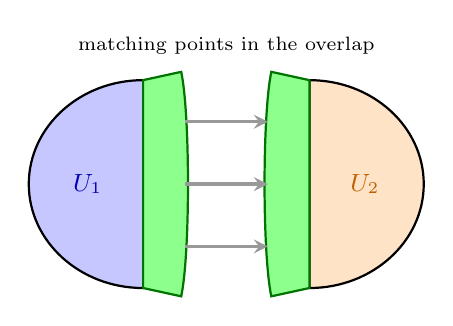
\begin{tikzpicture}[>=stealth, scale=0.88]
  % Two overlapping open patches, each with a collar along its full flat edge
  \draw[thick, fill=blue!22] (-1.2,1.5) arc (90:270:1.65 and 1.5) -- cycle;
  \path[fill=green!45, draw=green!45!black, thick]
    (-1.2,1.5) -- (-1.2,-1.5) -- (-0.65,-1.62)
    .. controls (-0.52,-1.0) and (-0.52,1.0) .. (-0.65,1.62) -- cycle;

  \draw[thick, fill=orange!22] (1.2,1.5) arc (90:-90:1.65 and 1.5) -- cycle;
  \path[fill=green!45, draw=green!45!black, thick]
    (1.2,1.5) -- (1.2,-1.5) -- (0.65,-1.62)
    .. controls (0.52,-1.0) and (0.52,1.0) .. (0.65,1.62) -- cycle;

  \node[font=\small, text=blue!70!black] at (-2.0,0) {$U_1$};
  \node[font=\small, text=orange!75!black] at (2.0,0) {$U_2$};
  \node[font=\scriptsize] at (0,2.0) {matching points in the overlap};

  % Arrows pair points all along the two full-edge overlap collars
  \draw[->, very thick, gray!80] (-0.6,0.9) -- (0.6,0.9);
  \draw[->, very thick, gray!80] (-0.6,0) -- (0.6,0);
  \draw[->, very thick, gray!80] (-0.6,-0.9) -- (0.6,-0.9);
\end{tikzpicture}

        \caption{%
            Two hemispherical patches, with matching green overlap strips.
            Arrows show corresponding points being mapped from the left strip
            to the right.
        }
        \label{fig:sphere_transition}
    \end{figure}

    \subsection{The Benefit: Uniting Local Calculus with Global Coherence}
    Why is this definition so effective?
    \begin{itemize}
        \item \textbf{Locally}:\\
            We can calculate using standard multivariable calculus from
            Section~\ref{sec:preliminaries} by pulling functions and vectors
            back to open subsets of $\mathbb{R}^n$ via charts. No new
            computational mechanics are needed.
        \item \textbf{Globally}:\\
            Because the transition maps $\psi \circ \phi^{-1}$ are smooth
            diffeomorphisms, the multivariate chain rule guarantees that all
            calculus operations (smoothness of functions, directional
            derivatives, vector fields, and differential forms) are
            coordinate-independent.
    \end{itemize}
    This allows us to study global derivatives, PDEs on curved geometries,
    optimization on manifolds, and global topological invariants (such as de
    Rham cohomology) rigorously.
